%!TEX root = ../../Main.tex
\graphicspath{{Chapters/Indledning/}}
%-------------------------------------------------------------------------------


\section{Teori}
I procceseringsfasen af projektet, har vi valgt at bruge et adaptivt filter - LMS (Least Mean square) algoritme. Et adaptivt filter består af 2 funktionelle blokke, hvor den ene blok fungerer som et filter, fra dynamiske kofficienter som bliver opdateret LMS blokken.  Filteret trækker herefter de beregnede filter fra det samlede lydsignal. 
   

\begin{figure}[H]
	\centering
	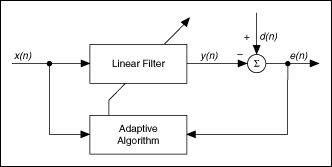
\includegraphics[width = 400pt]{Img/Figures}
	\caption{LMS adaptive filter}
	\label{fig:LMS_filter}
\end{figure}

På figur \ref{fig:LMS_filter} ses et overblik over det adative system, hvor x(n) er støjsignalet, y(n) er det filtrede støjsignal, med koefficienter som opdateres fra blokken "Adaptive Algoritm". d(n) er det ønskede signal inklusiv det støjende signal. e(n) er forskellen mellem d(n) og y(n) og derved støjen fratrukket fra det samlede signal af ønsket og støj.  \newline


Det digitale filter bliver beregnet ud fra formlen:

\begin{equation}
  y(n) = \displaystyle\sum_{l=0}^{L-1} W(n)*x(n-1)
\end{equation}
Hvor W(n) er den værdi, som dynamisk opdateres. Dette sker ved at vi beregner den næste værdi ud fra formlen: 
\begin{equation}
  W(n+1) = W(n)-\mu *X(n)*e(n)
\end{equation}

Hvor W er den nye koefficient til filteret, X(n) er input signalet, og \textmu\ er en faktor, som bestemmer hastigheden af filteret, samt styrer infaldstiden. Hvis \textmu\ er lav bliver filteret langtsommere, mens settling time stiger jo højere vi kommer. Typisk må denne værdi ikke overstige 1. 
\newline
Dette giver os et endeligt udtryk som stemmer overens med figur \ref{fig:LMS_filter}, ift summeringspunktet: 
\begin{equation}
  e(n) = d(n)-y(n)
\end{equation}